\begin{figure}
The system is classified into several service models, admin can enable/disable any 
of these services via the Service interface from the administration menu based on 
the clients’ requirements. For example, admin can simply uncheck the OntoService 
and click on the Save button, then the OntoService will be removed from the current 
installation.
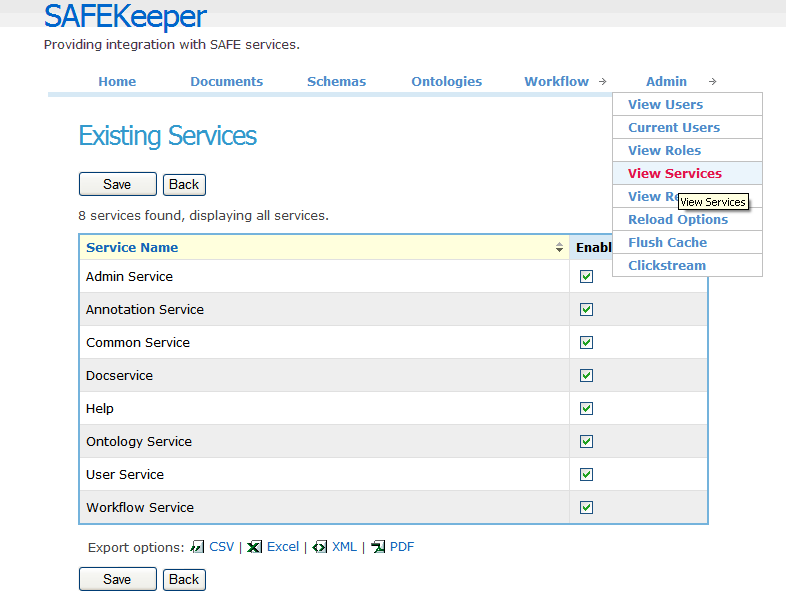
\includegraphics[scale=0.4]{servicelist}
\caption{Existing Services}
\label{fig:servicelist}
\end{figure}

\begin{figure}
Similar to the role management, administrator can manage all the resources 
(URLs within the system) via the resource management page. Basically, each URL 
is assigned to one or several existing roles so that only users with certain roles 
can have the access to the specific resources. Each resource belongs to a service. 
The light icons will be off when a service is disabled and on once a service is 
enabled again. However, you need to reassign the roles for each resource after 
you re-enable a service to make the resources work properly.
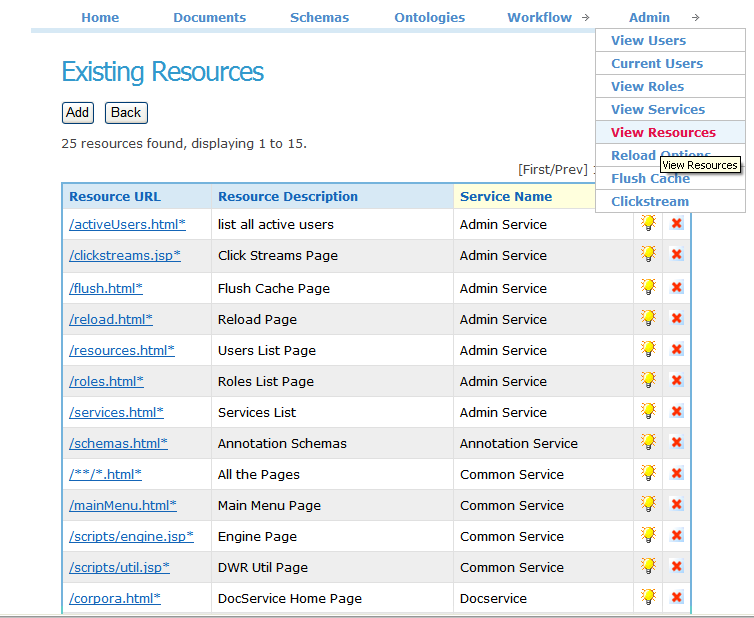
\includegraphics[scale=0.4]{resourcelist}
\caption{Existing Resources}
\label{fig:resourcelist}
\end{figure}

\begin{figure}
To refresh the cache in the system, administrator can simply click on the Flush 
in the Administration menu.
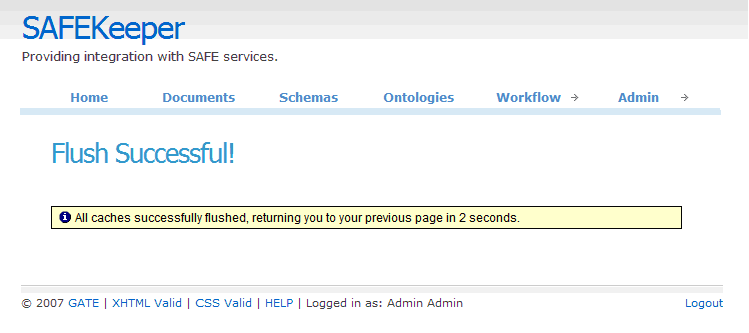
\includegraphics[scale=0.4]{flush}
\caption{Flush Cache}
\label{fig:flush}
\end{figure}